%------------------------------------------------
% 		LEVEL 1
%------------------------------------------------
\subsection*{Level 1}
\addcontentsline{toc}{subsection}{Level 1}

The embedded Matlab implementation leads to the exact same result than the implementation using ordinary Simulink blocks. Indeed, since we use a discretize controller, transposing the simulink code to the embedded Matlab implementation produce the a code with the same behavior as the one produced by Simulink.

Figure \ref{embedded} show the superposition of the embedded implementation and the one using Simulink.


\begin{figure}[ht]
  \centering
  \begin{subfigure}[b]{\linewidth}
   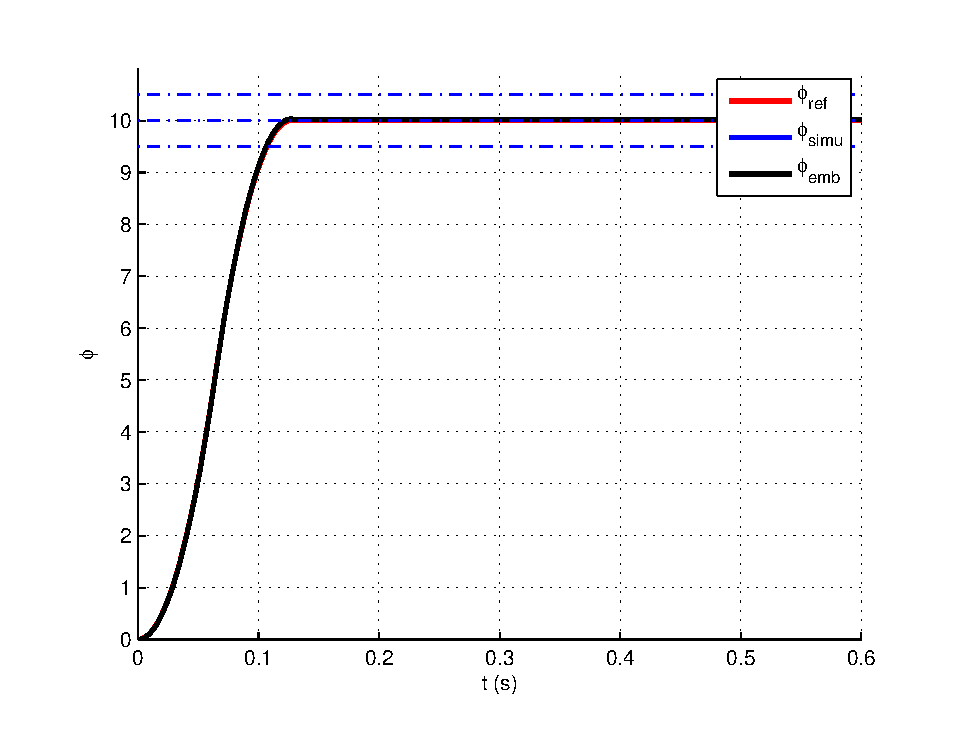
\includegraphics[width=\columnwidth]{fig/embeddedlvl110.eps}
   \caption{$Rs = 10$[rad]}
  \end{subfigure}
  \begin{subfigure}[b]{\linewidth}
  \includegraphics[width=\columnwidth]{fig/embeddedlvl1100.eps}
   \caption{$Rs = 100$[rad]}
  \end{subfigure}

 \caption{Result with a embedded controller}
 \label{embedded}
\end{figure}

%------------------------------------------------
% 		LEVEL 2
%------------------------------------------------
\subsection*{Level 2}
\addcontentsline{toc}{subsection}{Level 2}
